

\tikzset{every picture/.style={line width=0.75pt}} %set default line width to 0.75pt        

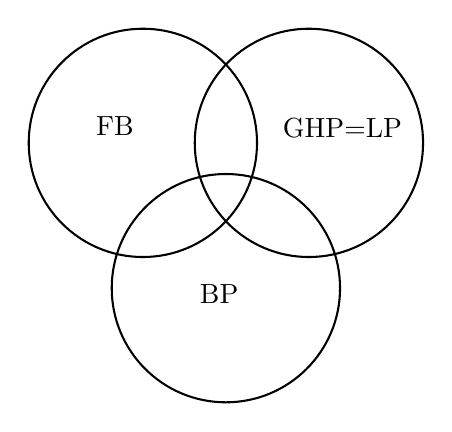
\begin{tikzpicture}[x=0.75pt,y=0.75pt,yscale=-1,xscale=1]
%uncomment if require: \path (0,300); %set diagram left start at 0, and has height of 300

%Shape: Circle [id:dp5565937779986971] 
\draw   (90,65) .. controls (90,34.62) and (114.62,10) .. (145,10) .. controls (175.38,10) and (200,34.62) .. (200,65) .. controls (200,95.38) and (175.38,120) .. (145,120) .. controls (114.62,120) and (90,95.38) .. (90,65) -- cycle ;
%Shape: Circle [id:dp3604112362399041] 
\draw   (50,135) .. controls (50,104.62) and (74.62,80) .. (105,80) .. controls (135.38,80) and (160,104.62) .. (160,135) .. controls (160,165.38) and (135.38,190) .. (105,190) .. controls (74.62,190) and (50,165.38) .. (50,135) -- cycle ;
%Shape: Circle [id:dp341505309398217] 
\draw   (10,65) .. controls (10,34.62) and (34.62,10) .. (65,10) .. controls (95.38,10) and (120,34.62) .. (120,65) .. controls (120,95.38) and (95.38,120) .. (65,120) .. controls (34.62,120) and (10,95.38) .. (10,65) -- cycle ;

% Text Node
\draw (41,51) node [anchor=north west][inner sep=0.75pt]   [align=left] {FB};
% Text Node
\draw (131,52) node [anchor=north west][inner sep=0.75pt]   [align=left] {GHP=LP};
% Text Node
\draw (91,132) node [anchor=north west][inner sep=0.75pt]   [align=left] {BP};


\end{tikzpicture}
